\section{FORMATIONS}

\subsection{Formations}

At all times the \textbf{wingman is responsible for flight path deconfliction
and visual lookouts}.  Lead can step down by directing "2, you have lead" At
which point the WM will take over the FL position and report, "2 has lead". This
does not imply a callsign change, just a lead aircraft change for navigation and
formation purposes.

Loss of Visual or "Blind" Procedures: Flight members will call "blind" with
their altitude in thousands of feet, e.g. "X, blind angels 15.2". A visual
flight member will call "visual" and initiate a talk-on to achieve
deconfliction and allow the blind pilot to visually re-acquire the flight. If
both flight members are blind, they will both call "blind" and proceed to move
according to contract "Lead Left, High, Wingman Right and Low" and step up/down
1000ft and separate heading 10 degrees.

Yardstick should be referred to for deconfliction and rejoin.

\subsection{En Route Formations}

\sidebyside{0.5}{%
  Standard En Route formation contract is Echlon for a 2-ship and Finger Four
  for a four-ship. The standard side would be Left (mirroring positions on the
  deck, -2 on the right, -3 and -4 on the left) until changed by FL. The sole
  task of the wingman is to maintain formation flight.

  The sight lines should have the Pilot looking at the leads Engine intakes at
  90 degrees and stepped down to be level with the belly. Consider alternating
  sides for a break or pushing out to a more comfortable cruise setting.
}{%
  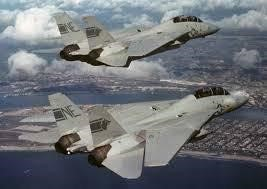
\includegraphics[width=\textwidth,align=t]{formations/enroute}%
}

\subsubsection{Finger Four}

\sidebyside{0.5}{%
  The finger four is the standard close formation configuration and is so named
  after the likeness to the fingertips on your hand. Finger Four can be flown
  strong right or strong left, as desired by the Flight Lead. The term
  "fingertip", if used during four ship operations, refers to the "finger four"
  formation.

  The finger formation is a transit formation and is not used in a combat. The
  formation is ideal for penetrating clouds since the close proximity of
  aircraft allow sight to be maintained.
}{%
  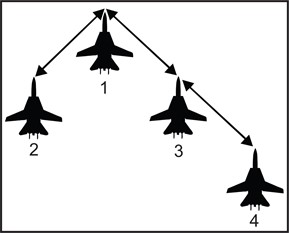
\includegraphics[width=\textwidth,align=t]{formations/finger-four}%
}

\subsubsection{Echelon Formation}

\sidebyside{0.5}{%
  The echelon four ship formation can either be formed right or left. The
  flight lead will either call "echelon left/right". The echelon formation will
  be used during the CASE I \& II recoveries. Echelon formation is a transit
  formation and not used in combat.
}{%
  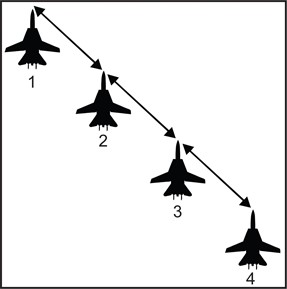
\includegraphics[width=\textwidth,align=t]{formations/echelon}%
}

\subsection{Tactical Formations}

Tactical formations are formations where the lead and wingman are separated by
0.5 nm or more. The intended flow of the flight will be called out by the lead.
They are used after Fencing In for best weapons employment.

\subsubsection{Combat spread Formation / \color{red}{Line Abreast}}

Combat spread refers to a section employing offensively to known threats from a
specific axis. Wing will fly abeam, 1.0 to 1.5 nm, up to 3,000 ft above or
below Lead's altitude. The combination of these parameters may be varied based
upon environmental factors (sun angle, atmospherics, terrain, etc.) so the
Fighters can remain mutually supportive and hopefully diminish the ability of
the Bandit to gain sight of either or both of the Fighters.

\begin{center}
  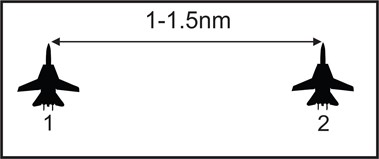
\includegraphics[width=0.75\textwidth,align=t]{formations/combat-spread}
\end{center}

\subsubsection{Wedge Formation}

\sidebyside{0.5}{%
  The wedge formation is a tactical formation that can be used as a two ship or
  four ship formation. The formation provides excellent offence ahead of the
  3/9-line, inexperienced wingmen may find it easier to stay in position and
  can be used in low level flight in rugged terrain. The formation offers poor
  6 o'clock lookout. A single threat can affect the entire flight.
}{%
  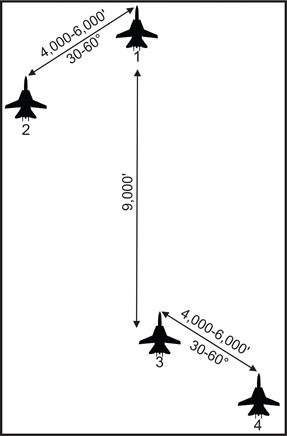
\includegraphics[width=\textwidth,align=t]{formations/wedge}%
}

\subsubsection{Four-Ship Fighting Wing}

\sidebyside{0.5}{%
  The four-ship fighting wing offers the same benefits as the two-ship fighting
  wing. In a scenario where the flight lead is manoeuvring quicky for example,
  during a tanker rejoin. The four-ship fighting wing allows the formation to
  remain with the flight lead
}{%
  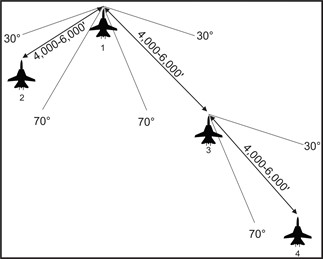
\includegraphics[width=\textwidth,align=t]{formations/fighting-wing}%
}


\subsubsection{Box \& Offset Box}

\sidebyside{0.5}{%
  The box \& offset box formation is a tactical formation that provides good
  mutual support and makes it difficult to visually acquire the entire flight.
  The element spacing for attack is built into the formation. The formation is
  not suited to low level flying in rugged terrain. Depending on the position
  the trailing element can be mistaken as a threat.
}{%
  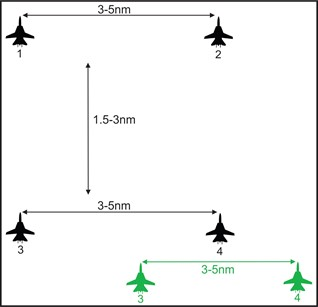
\includegraphics[width=\textwidth,align=t]{formations/box}%
}

\subsubsection{Four}

The fluid four formation is a tactical formation that offers good
manoeuvrability for the whole formation and concentration of force. The
formation can be engaged simultaneously and going defensive can become
confusing because of the proximity of the other aircraft. The formation should
not be used at low altitude with rough terrain

\begin{center}
  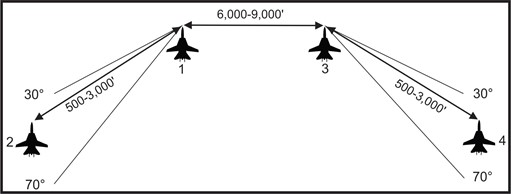
\includegraphics[width=0.75\textwidth,align=t]{formations/fluid}%
\end{center}


\subsubsection{Spread Four}

The spread four is a tactical formation that is ideal for BVR engagements. The
lateral spacing allows for maximum airspace control while still being able to
provide mutual support. The formation is not suited for low level flying in
rough terrain and it can be difficult for the wingmen to maintain formation
while manoeuvring.

\begin{center}
  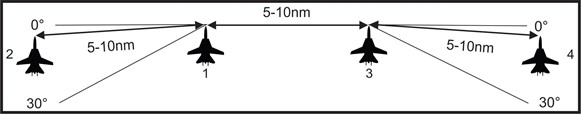
\includegraphics[width=0.75\textwidth,align=t]{formations/spread-four}%
\end{center}


\subsubsection{Trail}

\sidebyside{0.5}{%

  Trail is a tactical formation where the wingman trails the flight lead at a
  distance of 2-4nm. Transitioning from Trail is done by manoeuvring, not by
  slowing down the trailing aircraft. Transition to Trail as follows:

  \begin{enumerate}

    \item Turn 90\textdegree~off course

    \item Maintain course for \sfrac{1}{2} the distance ordered for Trail

    \item Turn 180\textdegree

    \item Turn to Trail on original heading

  \end{enumerate}

  Transition to trail should be used using TACAN to get accurate distances.

  In step 2, begin the turn a few seconds before reaching exactly \sfrac{1}{2}
  the distance, because the 180\textdegree~turn takes some time.

}{%
  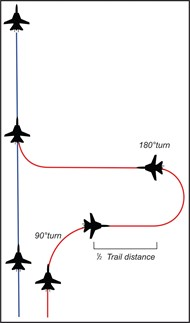
\includegraphics[width=\textwidth,align=t]{formations/trail}%
}

\newpage

\subsection{Turns}

Tactical turns are required to \textbf{preserve spacing} whilst aircraft are
separated by larger distances in tactical formation. In \textbf{Hook} and
\textbf{Cross Turns}, both aircraft turn simultaneously. In all other Tactical
turns the \textbf{outside} aircraft \textbf{always} crosses the path of the
\textbf{inside} aircraft during the turn, and the inside aircraft turns when
the outside aircraft's nose/tail points at it. All tactical turns are flown at
MIL power.

After the turn is complete the throttle is returned to its position before the
turn commenced. The airspeed and altitude before, during, and after the turn
must remain constant. The following procedure is required: An \textbf{energy
sustaining turn} is a level turn conducted at full military power using "G" to
\textbf{maintain} airspeed.

\begin{itemize}

  \item Set throttle to FULL MIL

  \item Bank and pull to maintain a level turn at exactly the contract speed
    (for example 350 knots)

  \item At your new heading roll out back to level

  \item Return the throttle to the position it was before the turn and ensure
    you are still at your briefed speed.

\end{itemize}


\subsubsection{90\textdegree Tactical Turns}

\sidebyside{0.5}{%

  A 90\textdegree tactical turn will be directed with the call "TAC Left /
  Right 90/45" or "TAC Left / Right heading". The turn will start immediately
  when the last pilot responds with their flight number.

  The pilot that is turning into their wingman initiates the turn by turning
  first. In other words, any maybe easier to remember, \textbf{the pilot flying
  outside of the turn, will turn first.}

  When turning away from the wingman the pilot will watch the other airframe
  begin its turn and then initiate their own turn when the other airframe's
  nose is pointing directly at them.

  Both aircraft will complete the turn by performing an \textbf{energy
  sustained} turn.
}{%
  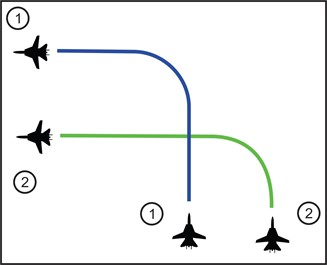
\includegraphics[width=\textwidth,align=t]{turns/tac-90}%
}

\subsubsection{45\textdegree Tactical Turns}

\sidebyside{0.5}{%

  A 45\textdegree tactical turn while in line abreast formation will be
  directed with the call "SPECTRES TAC45left/right". The turn will start
  immediately when the last pilot responds with their fight number. When
  turning away from the wingman the pilot will watch the other airframe begin
  it's turn and then initiate their own turn when the other airframe passes
  their 6 o'clock position. Both aircraft will perform the turn by performing
  an energy sustained turn

}{%
  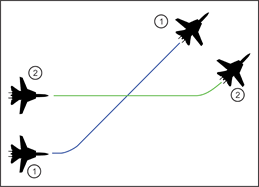
\includegraphics[width=\textwidth,align=t]{turns/tac-45}%
}


\subsubsection{30\textdegree Check Turns}

\sidebyside{0.5}{%

  A 30\textdegree check turn while in line abreast formation will be directed
  with the call "Check Left / Right" or "Check Left / Right heading".  The turn
  will start immediately when the last pilot responds with their flight number.
  Both aircraft initiate the turn simultaneously to maintain a 30\textdegree
  bank.  The inside aircraft turns an additional 30\textdegree then turns back
  to re-establish the 1 NM spacing. This snaking maneuver prevents the inside
  pilot from moving ahead and breaking the line-abreast formation.

  The throttle must be used to ensure airspeed remains constant throughout the
  manoeuvre.

}{%
  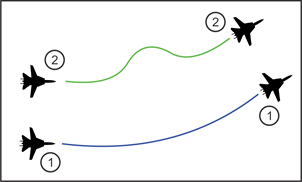
\includegraphics[width=\textwidth,align=t]{turns/check-30}%
}



\subsubsection{Hook Turns}

\sidebyside{0.5}{%
  A hook turn allows the flight to reverse direction while maintaining
  formation.

  The flight lead will call "SPECTRES hook right/left".

  The turn is an energy sustaining turn. Both aircraft initiate a
  simultaneously level energy sustained turn which continues until the airframe
  is pointing in the reciprocal direction. During the turn, the trail aircraft
  at the 90 can check the other's aircraft aspect \& increase or decrease the G
  load to maintain position.


}{%
  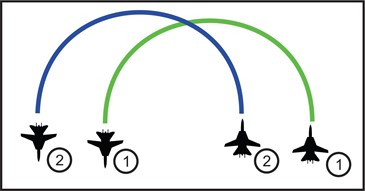
\includegraphics[width=\textwidth,align=t]{turns/hook}%
}

\subsubsection{Cross Turn}

\sidebyside{0.5}{%
  A cross turn allows the flight to reverse their direction while maintaining
  their tactical formation. The turn will start immediately when the last pilot
  responds with their flight number. Both aircraft initiate a simultaneous
  level energy sustained turn which continues until the airframe is pointing in
  the reciprocal direction.

  Note that because this turn typically starts 1 nm apart the aircraft are
  turning into each other. As the radius of a 180\textdegree energy sustaining
  turn has a much larger radius the aircraft will be substantially further than
  1 nm apart after the turn. Therefore, both aircraft should continue the turn
  for an additional 30\textdegree, and then turn back to the desired heading
  once their separation gets to 1.4 nm to settle on the final heading at 1 nm.

}{%
  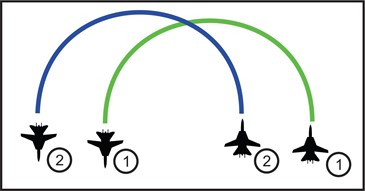
\includegraphics[width=\textwidth,align=t]{turns/cross}%
}

\subsubsection{Shackle}

\sidebyside{0.5}{%
  A shackle maneuver is used to switch sides. It can also be a quick way to get
  two aircraft no longer abreast back into position.  The turn will start
  immediately when the last pilot responds with their flight number.  The two
  aircraft initiate a 45\textdegree turn into each other.  Once the wingman
  passes over the lead pilot the two aircraft start to turn back toward the
  original heading so as to end up with the correct tactical spacing between
  the two aircraft.
}{%
  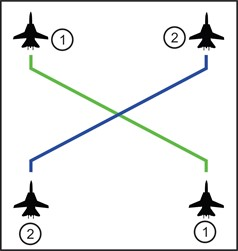
\includegraphics[width=\textwidth,align=t]{turns/shackle}%
}

